\documentclass[a4paper]{article} %% Classe do documento
\usepackage[margin=2cm]{geometry} %% Dimens?es das margens
\usepackage[utf8]{inputenc}
\usepackage[T1]{fontenc}
\usepackage[brazil]{babel}
\usepackage{graphicx}
\usepackage{verbatim}
\usepackage{alltt}
\usepackage{here}
\usepackage{xcolor}
\usepackage{fancyhdr}
\usepackage{setspace}
\usepackage{indentfirst}
\usepackage{multirow}
\usepackage{makeidx}
\usepackage{wrapfig}
\usepackage[all]{xy}
\usepackage{fancybox}
\usepackage{rotating}
\usepackage{eso-pic}
\usepackage{dcolumn}
\usepackage{color}
\usepackage{lscape}
\usepackage{subfigure}
\usepackage{scalefnt}

\newcommand{\undertilde}[1]{\underset{\widetilde{}}{#1}}

\usepackage{Sweave}
\begin{document}
\Sconcordance{concordance:count1.tex:count1.Rnw:%
1 28 1 1 0 47 1 1 2 1 0 3 1 1 4 8 0 1 5 1 3 2 0 2 1 5 0 1 3 1 1 1 4 3 0 %
8 1 4 0 1 2 1 1 1 2 1 0 8 1 4 0 1 2 3 1 1 2 15 0 4 1 4 0 1 2 5 1 1 2 1 %
0 1 2 2 1 4 0 1 2 7 1}

\begin{titlepage}

  \center{\rule{15cm}{2pt}}
  \begin{center}{\bf Universidade Federal do Paran?\\
      Departamento de Estat?stica\\[8cm]

      {\large
        Regress?o para Dados de Contagem - Mortalidade em Santa Catarina ano de 2016}\\[2cm]

      { CE225 - Modelos Lineares Generalizados}\\[5cm]

      { La?s Hoffmam GRR201}
      
      { Simone Matsubara GRR20124663}
      
      { Willian Meira GRR201}

      { Yasmin Fernandes GRR201}

      % \end{minipage}
      \vfill
      Curitiba, 24 de Novembro de 2018
      \center{\rule{15cm}{2pt}}}
  \end{center}
\end{titlepage}

\tableofcontents
\pagebreak

\section{Introdu??o}

kkkk


\section{Material e M?todos}
\subsection{Material}




\subsection{M?todos}

contagem

\section{An?lise Descritiva}

\begin{Schunk}
\begin{Sinput}
> library(ggplot2)
> library(gridExtra)
> library(corrplot)
> library(readxl)
> dados <- read_xls('Base_fim.xls',
+                   col_types = c("text", "numeric", "numeric","numeric", "numeric",
+                                 "numeric","numeric", "numeric", "numeric"))
> 
> 
> 
\end{Sinput}
\end{Schunk}

\begin{Schunk}
\begin{Sinput}
> # Quantidade de munic?pios por total de incid?ncia
> tabobt <- table(dados$obit)
> tabpobt <- table(round(dados$obit/sum(dados$obit)*100, digits = 2))
> barplot(tabobt)
> 
\end{Sinput}
\end{Schunk}
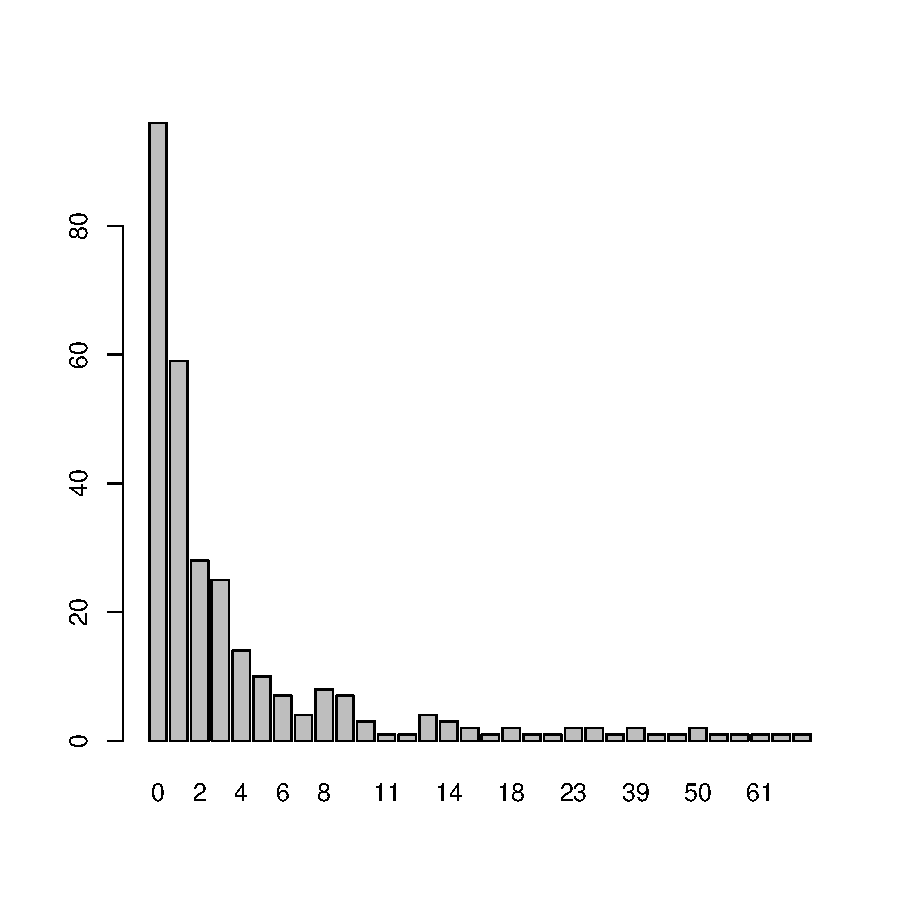
\includegraphics{count1-002}


\begin{Schunk}
\begin{Sinput}
> #Boxplots
> 
> par(mfrow=c(3,3))
> boxplot(dados$obit, xlab = '', ylab = '', main = '?bitos no Tr?nsito', las=1)
> boxplot(dados$vphab, xlab = '', ylab = '', main = 'Ve?culos a cada 100 Habit', las=1)
> boxplot(dados$dens, xlab = '', ylab = '', main = 'Densidade Demogr?fica', las=1)
> boxplot(dados$purb, xlab = '', ylab = '', main = '% Pop Urbana', las=1)
> boxplot(dados$palf, xlab = '', ylab = '', main = '% Alfabetizados', las=1)
> boxplot(dados$pdes, xlab = '', ylab = '', main = '% Desmpregados', las=1)
> boxplot(dados$rmed, xlab = '', ylab = '', main = '% Pop Baixa Renda', las=1)
> boxplot(dados$idh, xlab = '', ylab = '', main = 'IDH', las=1)
\end{Sinput}
\end{Schunk}
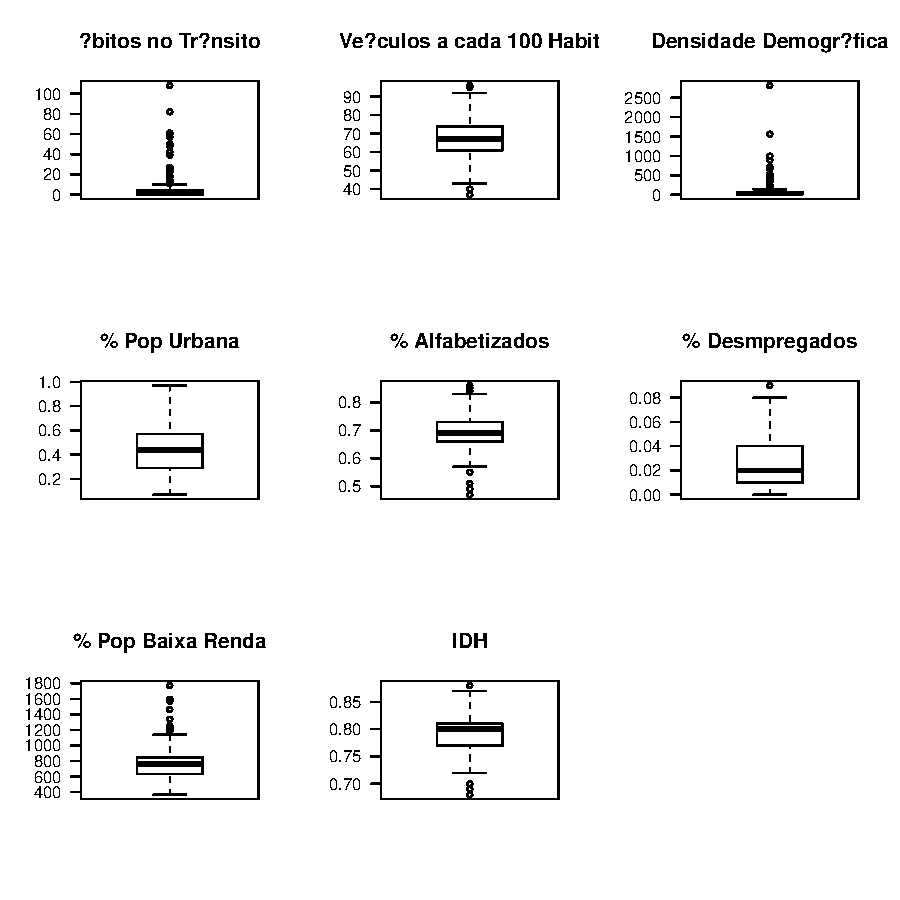
\includegraphics{count1-003}


\begin{Schunk}
\begin{Sinput}
> g1 <- ggplot(dados, aes(x=obit)) + geom_histogram()+ xlab('?bitos no Tr?nsito')+ ylab('')
> g2 <- ggplot(dados, aes(x=vphab)) + geom_histogram()+ xlab('Ve?culos a cada 100 Habit')+ ylab('')
> g3 <- ggplot(dados, aes(x=dens)) + geom_histogram()+ xlab('Densidade Demogr?fica')+ ylab('')
> g4 <- ggplot(dados, aes(x=purb)) + geom_histogram()+ xlab('% Pop Urbana')+ ylab('')
> g5 <- ggplot(dados, aes(x=palf)) + geom_histogram()+ xlab('% Alfabetizados')+ ylab('')
> g6 <- ggplot(dados, aes(x=pdes)) + geom_histogram()+ xlab('% Desmpregados')+ ylab('')
> g7 <- ggplot(dados, aes(x=rmed)) + geom_histogram()+ xlab('Renda M?dia')+ ylab('')
> g8 <- ggplot(dados, aes(x=idh)) + geom_histogram()+ xlab('IDH')+ ylab('')
> grid.arrange(g1, g2, g3, g4, g5, g6, g7, g8, ncol=3, nrow=3)
\end{Sinput}
\end{Schunk}
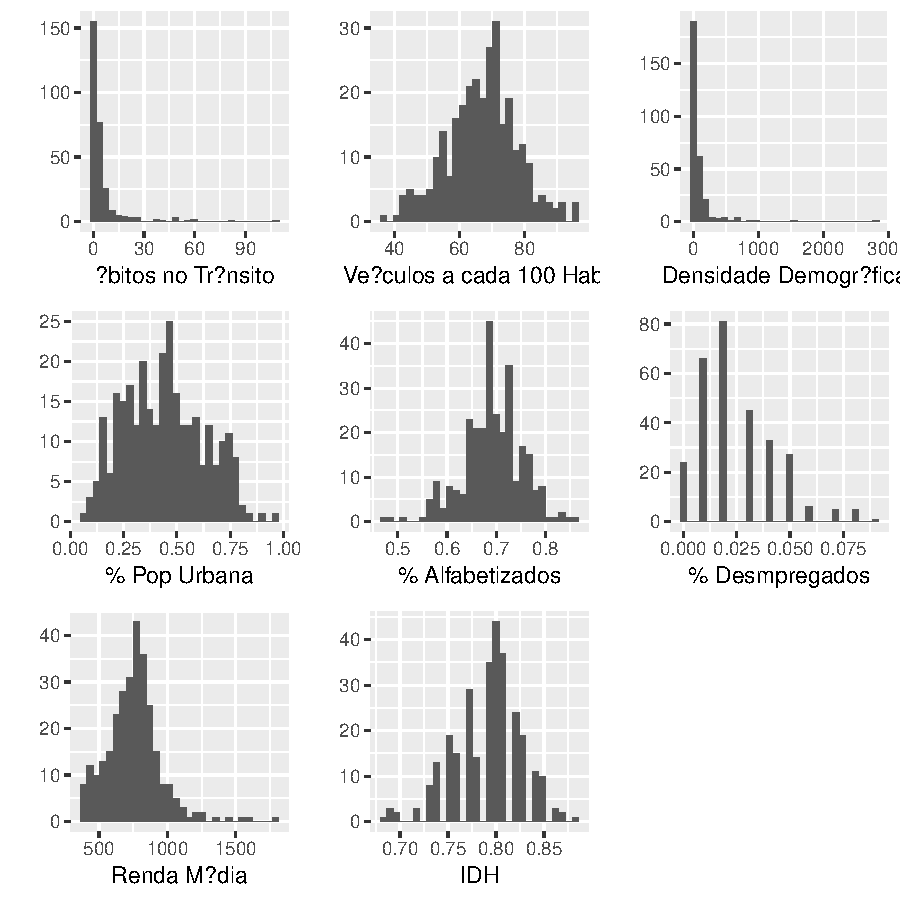
\includegraphics{count1-004}


Pelos boxplots e histogramas verificamos uma grande assimetria na covari?vel "Densidade Demografica". Vale a pena fazer uma transforma??o nesta vari?vel, para melhorar a assimetria aplicando log.

\begin{Schunk}
\begin{Sinput}
> str(dados)
\end{Sinput}
\begin{Soutput}
Classes ‘tbl_df’, ‘tbl’ and 'data.frame':	293 obs. of  9 variables:
 $ munic: chr  "Abdon Batista" "Abelardo Luz" "Agrolândia" "Agronômica" ...
 $ obit : num  0 4 1 3 10 3 0 8 6 0 ...
 $ vphab: num  65 56 72 70 63 55 83 74 67 72 ...
 $ dens : num  11.1 18.6 50.4 41.3 5.4 46.1 31.9 19 13.5 19.1 ...
 $ purb : num  0.27 0.41 0.44 0.16 0.44 0.34 0.22 0.28 0.25 0.26 ...
 $ palf : num  0.71 0.61 0.66 0.66 0.68 0.68 0.71 0.68 0.67 0.8 ...
 $ pdes : num  0.02 0.03 0.02 0.02 0.02 0.03 0.03 0.01 0.02 0.02 ...
 $ rmed : num  480 553 735 970 715 ...
 $ idh  : num  0.77 0.79 0.78 0.81 0.81 0.78 0.8 0.78 0.78 0.8 ...
\end{Soutput}
\begin{Sinput}
> dados$ldens  <- log(dados$dens)
> par(mfrow = c(1,2))
> hist(log(dados$dens), main = 'log(Densidade)', xlab = '', ylab = '')
> boxplot(log(dados$dens), xlab = '', ylab = '', main = 'log(Densidade)')
\end{Sinput}
\end{Schunk}
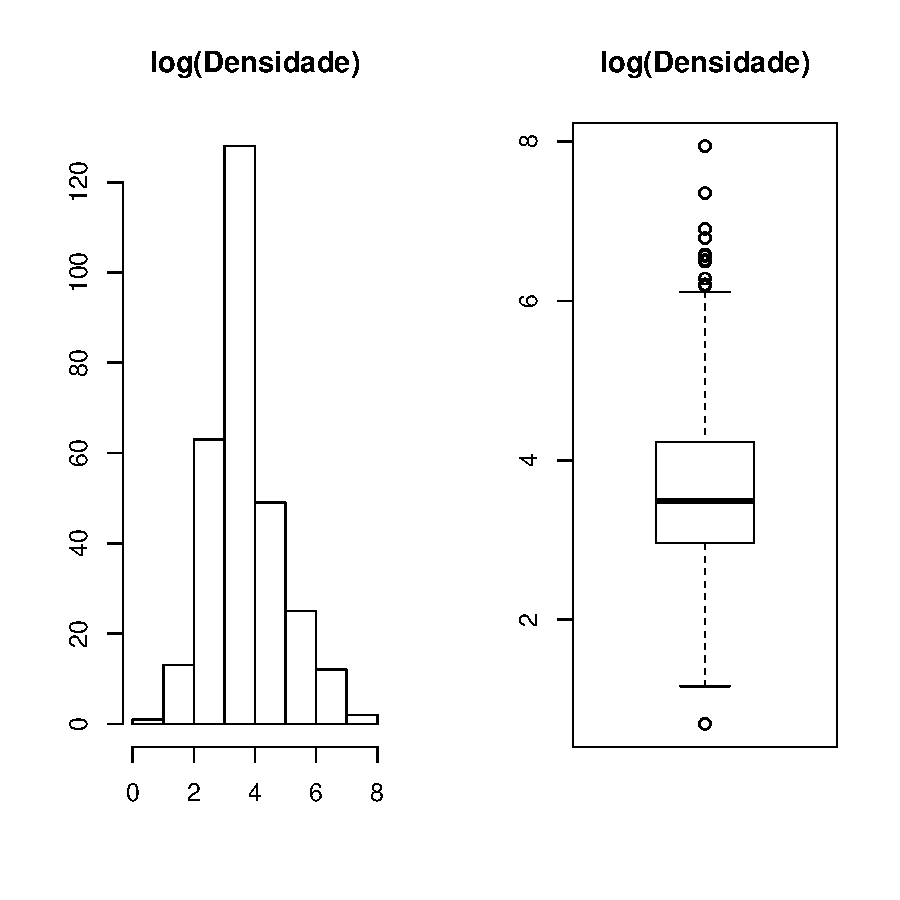
\includegraphics{count1-005}

Aplicando log, verificamos uma melhora consider?vel na assimetria dos dados da vari?vel


Vamos verificar a correla??o entre as vari?veis em estudo, substituino a vari?vel Densidade Demogr?fica pela log densidade.

\begin{Schunk}
\begin{Sinput}
> library(corrplot)
> cor <- cor(dados[ , c(2,3,10,5,6,7,8,9)])
> x11()
> corrplot.mixed(cor, upper = "ellipse")
\end{Sinput}
\end{Schunk}
\includegraphics{count1-006}



\section{Ajuste dos Modelos de Regress?o}



\end{document}
